\let\negmedspace\undefined
\let\negthickspace\undefined
\documentclass[journal]{IEEEtran}
\usepackage[a5paper, margin=10mm, onecolumn]{geometry}
%\usepackage{lmodern} % Ensure lmodern is loaded for pdflatex
\usepackage{tfrupee} % Include tfrupee package

\setlength{\headheight}{1cm} % Set the height of the header box
\setlength{\headsep}{0mm}     % Set the distance between the header box and the top of the text

\usepackage{gvv-book}
\usepackage{gvv}
\usepackage{cite}
\usepackage{amsmath,amssymb,amsfonts,amsthm}
\usepackage{algorithmic}
\usepackage{graphicx}
\usepackage{textcomp}
\usepackage{xcolor}
\usepackage{txfonts}
\usepackage{listings}
\usepackage{enumitem}
\usepackage{mathtools}
\usepackage{gensymb}
\usepackage{comment}
\usepackage[breaklinks=true]{hyperref}
\usepackage{tkz-euclide} 
\usepackage{listings}
% \usepackage{gvv}                                        
\def\inputGnumericTable{}                                 
\usepackage[latin1]{inputenc}                                
\usepackage{color}                                            
\usepackage{array}                                            
\usepackage{longtable}                                       
\usepackage{calc}                                             
\usepackage{multirow}                                         
\usepackage{hhline}                                           
\usepackage{ifthen}                                           
\usepackage{lscape}
\usepackage{circuitikz}
\usetikzlibrary{patterns}
\begin{document}
\bibliographystyle{IEEEtran}
\vspace{3cm}

\title{CE - 2021}
\author{EE24BTECH11064 - Harshil Rathan}
\maketitle

\renewcommand{\thefigure}{\theenumi}
\renewcommand{\thetable}{\theenumi}

\begin{enumerate}
\item Which of the following 1s/are correct statements(s)?
\begin{enumerate}
    \item Back Bearing of a line equal to Fore Bearing $\pm 180^\circ$.
    \item If the whole circle bearing of a line is $270^\circ$, its reduced bearing is $90^\circ NW$.
    \item The boundary of water of a calm water pond will represent contour line.
    \item In the case of fixed hair stadia tachometry, the staff intercept will be arger, when the staff is held nearer to the observation point.
\end{enumerate}
\item Consider the limit :
\begin{align*}
    \lim_{x\rightarrow 1}\brak{\frac{1}{\ln{x}}-\frac{1}{x-1}}
\end{align*}
The limit (correct up to one decimal place) is \underline{\hspace{1cm}} 
\vspace{0.5cm}

\item The volume determined from $\int\int\int_{V} 8xyz$ $dV$ for $V=[2,3]\times[1,2]\times[0,1]$ will be (in integer) \underline{\hspace{1cm}} 

\vspace{0.5cm}
\item The state of stress in a deformable body is shown in the figure. Consider transformation of the stress from the x-y coordinate system to the X-Y coordinate system. The angle $\theta$, locating the X-axis, is assumed to be positive when measured from the x-axis in counter clockwise direction.
\begin{figure}[H]
\centering
\resizebox{0.5\textwidth}{!}{%
\begin{circuitikz}
\tikzstyle{every node}=[font=\normalsize]
\draw [->, >=Stealth] (3,10) -- (3,15.25);
\draw [->, >=Stealth] (5.25,9.5) -- (5.25,8.5)node[pos=0.5, fill=white]{$\sigma_{yy}= 35.6 MPa$};
\draw [->, >=Stealth] (3,10) -- (9.25,10);
\draw [short] (8,10) -- (3,13.5);
\draw [->, >=Stealth] (5.25,12.75) -- (5.75,13.5)node[pos=0.5, fill=white]{$\sigma_{xx}=120 MPa$};
\draw [->, >=Stealth, dashed] (3,10) -- (6.25,15);
\draw [->, >=Stealth, dashed] (3,10) -- (0.5,11.5);
\draw [short] (4.5,12.75) -- (6,11.75);
\draw [short] (6,11.75) -- (5.75,12.25)node[pos=0.5, fill=white]{$\sigma_{xy}= 50 MPa$};
\draw [short] (4.5,9.75) -- (6.25,9.75);
\draw [short] (4.5,9.75) -- (5,9.5)node[pos=0.5, fill=white]{$\sigma_{xy}$};
\draw [short] (2.75,12.75) -- (2.75,11)node[pos=0.5,left, fill=white]{$\sigma_{xy}$};
\draw [short] (2.75,11) -- (2.5,11.5);
\draw [->, >=Stealth] (2.5,12) -- (1.5,12)node[pos=0.5,above, fill=white]{$\sigma_{xx}=40 MPa$};
\draw [->, >=Stealth] (3.75,10) .. controls (4.25,10) and (3.75,10.75) .. (3.25,10.5) node[pos=0.5, fill=white]{$\theta$};
\draw [short] (6.75,10) .. controls (6.25,10.25) and (6.75,10.75) .. (7.25,10.5)node[pos=0.5, fill=white]{$30^\circ$};
\draw [short] (3,14.75) -- (3,15);
\draw [short] (3,14.25) -- (3,15)node[pos=0.5,left, fill=white]{y};
\draw [short] (6,14.5) -- (6.25,15)node[pos=0.5,left, fill=white]{X};
\draw [short] (1,11.25) -- (0.75,11.5)node[pos=0.5,above, fill=white]{Y};
\draw [short] (8.5,10) -- (8.75,10);
\draw [short] (8.75,10) -- (9.25,10)node[pos=0.5,above, fill=white]{x};
\end{circuitikz}
}%

\end{figure}
The absolute magnitude of the shear stress component $\sigma_{xy}$( in MPa, round off to one decimal place) in x-y coordinate system is \underline{\hspace{1cm}} 
\vspace{0.5cm}
\item The equation od deformation is derived to be $y=x^2-xL$ for a beam shown in the figure.
\begin{figure}[H]
\centering
\resizebox{0.5\textwidth}{!}{%
\begin{circuitikz}
\tikzstyle{every node}=[font=\normalsize]
\draw [->, >=Stealth] (-0.25,12.25) -- (-0.25,15)node[pos=0.5,left, fill=white]{y};
\draw [short] (-0.25,12.25) -- (7,12.25);
\draw [short] (-0.25,12.25) -- (-0.25,11.5);
\draw [short] (-0.25,11.5) -- (7,11.5);
\draw [short] (7,11.5) -- (7,12.25);
\draw [dashed] (-0.25,12) -- (7,12);
\draw [dashed] (-0.25,12) .. controls (4,10.75) and (3.5,11) .. (7,12);
\draw [<->, >=Stealth] (0.25,8.75) -- (6.5,8.75)node[pos=0.5,above, fill=white]{L};
\draw [->, >=Stealth] (7,12) -- (8.75,12)node[pos=0.5,above, fill=white]{x};
\draw [short] (-0.25,11.5) -- (-1,10);
\draw [short] (-1,10) -- (1,10);
\draw [short] (1,10) -- (-0.25,11.5);
\draw [short] (-1,10) -- (-0.5,9.75);
\draw [short] (-0.5,10) -- (0,9.75);
\draw [short] (0,10) -- (0.5,9.75);
\draw [short] (0.5,10) -- (1,9.75);
\draw [short] (7,11.5) -- (6,10);
\draw [short] (6,10) -- (8,10);
\draw [short] (8,10) -- (7,11.5);
\draw  (6.25,9.75) circle (0.25cm);
\draw  (7,9.75) circle (0.25cm);
\draw  (7.75,9.75) circle (0.25cm);
\draw [short] (5.75,9.5) -- (8.25,9.5);
\draw [short] (5.75,9.5) -- (6.25,9.25);
\draw [short] (6.25,9.5) -- (6.75,9.25);
\draw [short] (6.75,9.5) -- (7.25,9.25);
\draw [short] (7.25,9.5) -- (7.75,9.25);
\draw [short] (7.75,9.5) -- (8.25,9.25);
\draw [short] (0.25,9) -- (0.25,8.5);
\draw [short] (6.5,9) -- (6.5,8.5);
\end{circuitikz}
}%

\end{figure}
The curvature of the beam at the mid-span (in units, in integer) will be \underline{\hspace{1cm}} 
\vspace{0.5cm}
\item The truss $EFGH$ is shown in the figure, in which all the members have the same axial rigidity R. In the figure, P is the magnitude of external horizontal forces acting at joints $F$ and $G$
\begin{figure}[H]
\centering
\resizebox{0.55\textwidth}{!}{%
\begin{circuitikz}
\tikzstyle{every node}=[font=\normalsize]
\draw [short] (-0.25,11.5) -- (7,11.5);
\draw [short] (-0.25,11.5) -- (-1,10);
\draw [short] (-1,10) -- (1,10);
\draw [short] (1,10) -- (-0.25,11.5);
\draw [short] (-1,10) -- (-0.5,9.75);
\draw [short] (-0.5,10) -- (0,9.75);
\draw [short] (0,10) -- (0.5,9.75);
\draw [short] (0.5,10) -- (1,9.75);
\draw [short] (7,11.5) -- (6,10);
\draw [short] (6,10) -- (8,10);
\draw [short] (8,10) -- (7,11.5);
\draw  (6.25,9.75) circle (0.25cm);
\draw  (7,9.75) circle (0.25cm);
\draw  (7.75,9.75) circle (0.25cm);
\draw [short] (5.75,9.5) -- (8.25,9.5);
\draw [short] (5.75,9.5) -- (6.25,9.25);
\draw [short] (6.25,9.5) -- (6.75,9.25);
\draw [short] (6.75,9.5) -- (7.25,9.25);
\draw [short] (7.25,9.5) -- (7.75,9.25);
\draw [short] (7.75,9.5) -- (8.25,9.25);
\draw (-0.25,11.5) to[short, -o] (-0.25,16.25) node[above] {F};
\draw (-0.25,13.75) to[short, -o] (-0.25,11.5) node[left] {E};
\draw (7,11.5) to[short, -o] (7,16.25) ;
\draw (-0.25,16.25) to[short, -o] (7,16.25) node[above] {G};
\draw (7,14.25) to[short, -o] (7,11.5) node[right] {H};
\draw [short] (-0.25,16.25) -- (7,11.5);
\draw [short] (-0.25,8.5) -- (-0.25,8);
\draw [short] (7,8.5) -- (7,8);
\draw [<->, >=Stealth] (-0.25,8.25) -- (7,8.25)node[pos=0.5,above, fill=white]{L};
\draw [->, >=Stealth] (-0.25,16.25) -- (-1.25,16.25)node[pos=0.5,left, fill=white]{P};
\draw [->, >=Stealth] (7,16.25) -- (8,16.25)node[pos=0.5,right, fill=white]{P};
\draw [short] (9.75,16.25) -- (10.25,16.25);
\draw [short] (9.75,11.5) -- (10.25,11.5);
\draw [<->, >=Stealth] (10,16.25) -- (10,11.5)node[pos=0.5,right, fill=white]{L};
\end{circuitikz}
}%

\end{figure}
If $R=500\times 10^3 kN$, $P=150kN$ and $L=3m$, the magnitude of the horizontal displacement of joint G (in mm, round off to one decimal place) is \underline{\hspace{1cm}}
\vspace{0.5cm}
\item The cohesion (c), angle of internal friction ($\phi$) and unit weight ($\gamma$) of a soil are $15 kPa$, $20^\circ$ and $17.5 kN/m^3$, respectively. The maximum depth of unspported excavtaion in the soil (in m, round off to two decimal places) is \underline{\hspace{1cm}}
\vspace{0.5cm}

\item Two reservoirs are connected through a homogeneous and isotropic aquifer having hydraulic conductivity (K) of $25$m/day and effective porosity ($\eta$) of 0.3 as shown in the figure (not to scale). Ground water is flowing in the aquifer at the steady state.
\begin{tikzpicture}
    % Define the angle of rotation for the main rectangle
    \begin{scope}[rotate=-10]
        % Draw and fill the main rectangle with a pattern
        \fill[pattern=north east lines] (0,0) rectangle (4,2.5);
        \draw[thick] (0,0) rectangle (4,2.5);
        \fill[pattern=north east lines] (0,0) rectangle (4,-1.2);
        \fill[pattern=north east lines] (-2.5,-1.2) rectangle (7,-1.5);
    \end{scope}
    
    % Draw a small horizontal white box inside the inclined rectangle (without rotation)
    \fill[white] (1.25,1) rectangle (2.75,1.5);
    \draw[thick] (1.25,1) rectangle (2.75,1.5);
    \fill[white] (-2,-1.2) rectangle (-0.5,-1.8);
    \draw[thick] (-2,-1.2) rectangle (-0.5,-1.8);
    \node at (-1.25,-1.5) {\textbf{Aquifuge}};
    % Add the text "Aquiclude" in bold font inside the small box
    \node at (2,1.25) {\textbf{Aquiclude}};

    \fill[white] (0,-1) rectangle (0.5,-0.5);
    \node at (0.25,-0.75) {\textbf{5m}};
    \draw[->] (0.2,-0.45) -- (0.3,-0.05);
    \draw[->] (0.15,-1) -- (0.1,-1.25);
    \fill[white] (0.7,-0.5) rectangle (1.9,-1);
    \node at (1.3,-0.75) {\textbf{Aquifer}};

    \fill[white] (2.1,-0.75) rectangle (3.8,-1.5);
    \node at (3,-0.9) {\textbf{K=25m/day}};
    \node at (3,-1.3) {\textbf{$\eta=0.3$}};
    % Draw a horizontal line 3 cm to the left of the inclined rectangle
    \draw[thick] (-2.7,1.8) -- (0.3,1.8);
    \draw[thick] (4.05,0.05) -- (6.8,0.05);
    \draw[thick] (-1.7,-2.3) -- (4.8,-2.3);
    \node at (1.8,-2.5) {Datum};
    \draw[thick] (-2.7,-0.8) -- (6.75,-2.4);
    \draw[->] (-0.5,1) -- (-0.5,1.8);
    \node at (-0.5,0.75) {30m};
    \node at (-2,0.8) {Reservoir 1};
    \draw[->] (-0.5,0.5) -- (-0.5,-2.3);
    \draw[->] (4.5,-0.5) -- (4.5,0.05);
    \node at (4.5,-0.75) {10m};
    \node at (5.5,-0.2) {Reservoir 2};
    \draw[->] (4.5,-1) -- (4.5,-2.3) ;
    
    \draw[->] (0.7,-1.65) -- (-0.3,-1.5);
    \node at (1.25,-1.7) {2 km};
    \draw[->] (1.7,-1.8) -- (3.7,-2.15) ;
    
    % Draw dotted lines parallel to the larger rectangle, 2 cm below
    \draw[dotted] (0, 0) -- (-0.3, -1.5);
    \draw[dotted] (3.9, -0.7) -- (3.6, -2.2);
    \draw[dashed, thick] (-2.6,-0.75) -- (-1,-0.75) ;
    \draw[->] (-2.3,-0.3) -- (-2.3,-0.75);
    \node at (-1.8,-0.5) {$10^{\circ}$};
    \draw[->] (-2.3,-1.5) -- (-2.3,-0.9) ;

\end{tikzpicture}
If water in Reservoir 1 is contaminated then the time (in days, round off to one decimal place)taken by the contaminated water to reach to Reservoir 2 will be \underline{\hspace{1cm}}
\vspace{0.5cm}
\item A signalized intersection operated in two phases. The lost time is 3 seconds per phase. The maximum ratios of approach flow to saturation flow for the two phases are 0.37 and 0.40. The optimum cycle length using the Webster's method (in seconds, round off to one decimal place) is \underline{\hspace{1cm}}
\vspace{0.5cm}
\item The solution of the second-order differential equation $\frac{d^2y}{dx^2}+2\frac{dy}{dx}+y=0$ with boundary conditions $y(0)=1$ and $y(1)=3$ is 
\begin{enumerate}
    \item $e^{-x}+(3e-1)xe^{-x}$
    \item $e^{-x}-(3e-1)xe^{-x}$
    \item $e^{-x}+[3e\sin{\frac{\pi x}{2}}-1]xe^{-x}$
    \item $e^{-x}-[3e\sin{\frac{\pi x}{2}}-1]xe^{-x}$
\end{enumerate}
\item The value of $\int_{0}^1 e^x dx$ using trapezoidal rule with four equal subintervals is 
\begin{enumerate}
    \item 1.718
    \item 1.727
    \item 2.192
    \item 2.718
\end{enumerate}  
\vspace{0.5cm}
\item A 50 ml, sample of industrial wastewater is taken into a silica crucible. The empty weight of the crucible is $54.352g$. The crucible with sample is dried in a hot air oven at $104^\circ$ till a constant weight of $55.129g$. Thereafter, the crucible with the dried sample is fired at $6006^\circ$ for 1h in a muffle furnace, and the weight of the crucible along with residue is determined as $54.783g$. The concentration of total volatile solids is \underline{\hspace{1cm}}
\begin{enumerate}
    \item 15540 mg/L
    \item  8620 mg/L
    \item 6920 mg/L
    \item 1700 mg/L
\end{enumerate}
\item A wedge M and a block N are subjected to forces \( P \) and \( Q \) as shown in the figure. If force \( P \) is sufficiently large, then the block N can be raised. The weights of the wedge and the block are negligible compared to the forces \( P \) and \( Q \). The coefficient of friction (\( \mu \)) along the inclined surface between the wedge and the block is 0.2. All other surfaces are frictionless. The wedge angle is \( 30^\circ \).
\begin{figure}[H]
\centering
\resizebox{0.6\textwidth}{!}{%
\begin{circuitikz}
\tikzstyle{every node}=[font=\normalsize]
\draw [short] (6,9) -- (14,9);
\draw [short] (7,9) -- (12.5,11.75);
\draw [short] (12.5,11.75) -- (12.5,9);
\draw [short] (8,9.5) -- (8,12);
\draw [short] (8,12) -- (10.75,12);
\draw [short] (10.75,12) -- (10.75,10.75);
\draw [->, >=Stealth] (14.5,10.5) -- (12.5,10.5);
\draw [->, >=Stealth] (9.25,14) -- (9.25,12);
\draw [->, >=Stealth] (11.75,12.25) .. controls (10.25,9.75) and (11,12.75) .. (9.75,10.5) ;
\draw [short] (8,9.5) .. controls (8.5,9.75) and (8.75,9) .. (8.25,9)node[pos=0.5,right, fill=white]{$30^\circ$};
\draw [short] (4.75,11) -- (8,11);
\draw [short] (8,11) -- (8,13.5);
\draw [short] (4.75,11) -- (5.25,11.25);
\draw [short] (5.25,11) -- (5.75,11.25);
\draw [short] (5.75,11) -- (6.25,11.25);
\draw [short] (6.25,11) -- (6.75,11.25);
\draw [short] (6.75,11) -- (7.25,11.25);
\draw [short] (7.25,11) -- (7.75,11.25);
\draw [short] (7.75,11) -- (8,11.25);
\draw [short] (8,13.5) -- (7.75,13);
\draw [short] (8,13.25) -- (7.75,12.75);
\draw [short] (8,13) -- (7.75,12.5);
\draw [short] (8,12.5) -- (7.75,12);
\draw [short] (8,12.75) -- (7.75,12.25);
\draw [short] (8,12.25) -- (7.75,11.75);
\draw [short] (8,12) -- (7.75,11.5);
\draw [short] (8,11.75) -- (7.75,11.25);
\draw [short] (8,11.5) -- (7.75,11);
\draw [short] (6,9) -- (6.5,8.75);
\draw [short] (6.5,9) -- (7,8.75);
\draw [short] (7,9) -- (7.5,8.75);
\draw [short] (7.75,9) -- (8.25,8.75);
\draw [short] (7.5,9) -- (7.75,8.75);
\draw [short] (8.25,9) -- (8.75,8.75);
\draw [short] (8.75,9) -- (9.25,8.75);
\draw [short] (9.25,9) -- (9.75,8.75);
\draw [short] (9.75,9) -- (10.25,8.75);
\draw [short] (10.25,9) -- (10.75,8.75);
\draw [short] (10.75,9) -- (11.25,8.75);
\draw [short] (11.25,9) -- (11.75,8.75);
\draw [short] (11.75,9) -- (12.25,8.75);
\draw [short] (12.25,9) -- (12.75,8.75);
\draw [short] (12.75,9) -- (13.25,8.75);
\draw [short] (13.25,9) -- (13.75,8.75);
\draw [short] (13.75,9) -- (14.25,8.75);
\draw [short] (11,9.25) -- (11,9.25)node[pos=0.5,above, fill=white]{Wedge M};
\node [font=\normalsize] at (8.75,11.5) {Block N};
\node [font=\normalsize] at (5.75,12.5) {Surface 3};
\node [font=\normalsize] at (9.75,8.25) {Surface 1};
\node [font=\normalsize] at (14.75,10.5) {P};
\node [font=\normalsize] at (9.25,14.25) {Q};
\node [font=\normalsize] at (12,12.75) {Surface 2};
\node [font=\normalsize] at (12.25,12.25) {$\mu$ =0.2};
\end{circuitikz}
}%

\end{figure}
The limiting force \( P \), in terms of \( Q \), required for impending motion of block \( N \) to just move it in the upward direction is given as \( P = \alpha Q \). The value of the coefficient \( \alpha \) (round off to one decimal place) is
\end{enumerate}
\end{document}

